\documentclass[PICOAPC.tex]{subfiles}

\begin{document}

%; see Tables~\ref{tab:specs} and \ref{tab:spec_bands}. 
\begin{wrapfigure}{R}{0.31\textwidth}  % r is right aligned, l is left. Capital letters allow figure to float on page.
\vspace{-5pt} % if move up and reduce to 12 lines only (add [12] before {R}) saves 1 line.
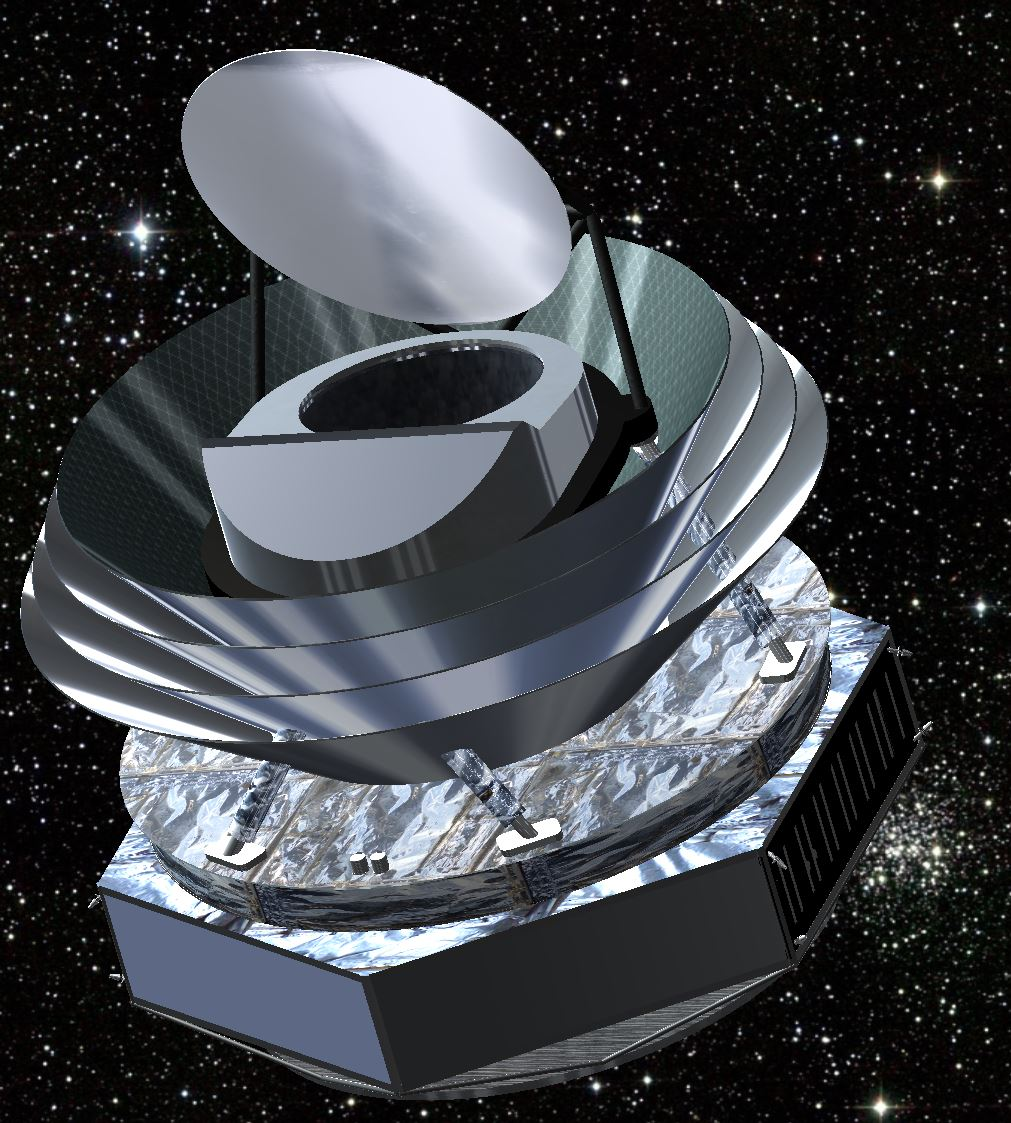
\includegraphics[width=0.31\textwidth]{images/PICO_Image.jpg}
\vspace{-0.25in}
\caption{\captiontext The PICO spacecraft 
\label{fig:pico_rendered} }
\end{wrapfigure}
The Probe of Inflation and Cosmic Origins (PICO, Fig.~\ref{fig:pico_rendered}) is an imaging polarimeter that will scan the sky for 5 years in 21 frequency bands spread between 21 and 799~GHz.
It will produce full-sky surveys of intensity and polarization with a final combined-map noise level equivalent to 3300 \planck\ missions for the baseline required specifications, and according to our current best-estimate 
would perform as 6400 \planck\ missions. With these capabilities, unmatched by any other existing or proposed platform: \\
$\bullet$ PICO could determine the energy scale of inflation and give a first, direct probe of quantum gravity by searching for the signal that arises from gravitational waves sourced by inflation and parameterized by the tensor-to-scalar ratio $r$. The PICO requirement is to reach $r =5\times10^{-4} \, (5\sigma)$, a level that is 100 times lower than current upper limits, and 5 times lower than limits forecast by any planned experiment.  If the signal is not detected, PICO is the only instrument that can exclude at $5 \sigma$\comred{(?)} models for which the characteristic scale in the potential is the Planck scale, a key threshold in inflation physics. \\ %\comred{cite swp} \\
$\bullet$ The mission will measure the minimum expected sum of the neutrino masses with $4\sigma$ confidence, rising to $7\sigma$ if the sum is near 0.1~eV. 
%Reaching the $4\sigma$ level can only be achieved with an instrument that can measure the polarization of the CMB on the largest angular scales {\it and} a measurement best done from space, which gives access to the full sky, and with a broad band of frequencies to remove foreground contaminants.  
PICO will give two additional independent and equally competitive constraints on the sum of neutrino masses. \\
$\bullet$ The measurements will either detect or strongly constrain deviations from the standard model of particle physics by counting the number of light particle species $N_{\rm eff}$ in the early universe with $\Delta N_{\rm eff} < 0.06 \, (2\sigma)$.  \\
$\bullet$ PICO will elucidate the processes affecting the evolution of cosmic structures by measuring the optical depth to reionization $\tau$ with an error $\sigma(\tau) = 0.002$, limited only by the small number of spatial modes available in the largest angular scale CMB polarization. \\
$\bullet$ Up to its resolution scale of few arcmin, the data will give a map of the projected gravitational potential due to all structures in the Universe with the highest \ac{SNR} relative to any foreseeable experiment, and it will give a catalog of 150,000 clusters extending to their earliest formation redshift. Each of these datasets will be used in combination with data from LSST and from future optical and infrared surveys to independently constrain the evolution of the amplitude of linear fluctuations $\sigma_{8}(z)$, with sub-percent accuracy.  \\
$\bullet$ PICO will determine the cosmological paradigm of the 2030s by reducing the allowed volume of uncertainty in a 12-dimensional $ \Lambda$CDM parameter space by a factor of nearly a billion relative to current \planck\ constraints on only six parameters. Such exquisite scrutiny will either give strong validation or require yet-to-be discovered revisions. \\
$\bullet$ PICO's maps of the Milky Way, which will have 3000 times more independent pixels compared to those available from Planck, will be used to resolve long-standing questions about our own Galaxy including the 
composition, temperature, and emissivities of Galactic dust, and the relative roles of gas turbulence and magnetic fields in the dynamics of the Galaxy and in the observed low star-formation efficiency. \\
$\bullet$ The data will constrain generic models of dark matter; enable a search for primordial magnetic fields with sufficient sensitivity to rule them out as the sole source for the largest observed galactic magnetic fields; constrain string theory motivated axions by improving by a factor of 300 constraints on polarization rotation arising from early Universe fields;  and will give precise tracing of the evolution with $z$ of thermal pressure in the universe through correlations of the thermal Sunyaev--Zeldovich effect with LSST's gold sample of galaxies, which will exceed a signal-to-noise ratio of 1000. 

\begin{wraptable}[38]{r}{0.45\textwidth}
\vskip -5mm
\hskip1.4cm
\begin{minipage}[t]{0.3\textwidth}
\caption{\textbf{Mission Parameters}\label{tab:specs}}
\begingroup
%\openup 5pt
\newdimen\tblskip \tblskip=5pt
\nointerlineskip
\vskip -5mm
\footnotesize %\footnotesize
\setbox\tablebox=\vbox{
    \newdimen\digitwidth
    \setbox0=\hbox{\rm 0}
    \digitwidth=\wd0
    \catcode`*=\active
    \def*{\kern\digitwidth}
%
    \newdimen\signwidth
    \setbox0=\hbox{+}
    \signwidth=\wd0
    \catcode`!=\active
    \def!{\kern\signwidth}
%
\halign{%
\hbox to 1.4in{#\leaderfil}\tabskip=0.6em plus 0.6em&
#\hfil\tabskip=0pt\cr
\noalign{\doubleline}
\multispan2 Combined polarization map depth$^{a}$ :\hfil\cr
\quad Baseline&0.87 $\mu$K$_{\rm CMB}$ arcmin\cr
\hskip1.75cm equivalent to 3300 \textit{Planck} missions\cr
\quad CBE$^{b}$&0.61 $\mu$K$_{\rm CMB}$ arcmin\cr
\hskip1.75cm equivalent to 6400 \textit{Planck} missions\cr
Survey duration / start & 5\,yrs / 2029 \cr
Orbit type & Sun-Earth L2 \cr
Launch mass & 2147\,kg \cr
Total power &1320\,W \cr
Data rate & 6.1\,Tbits/day \cr
Cost&\$\,958M\cr
%Launch&2029\cr
\noalign{\vskip 5pt\hrule\vskip 3pt}
\noalign{$^{a}$ rms noise in $1\times1$ arcmin$^{2}$ pixel.} % footnote to table
\noalign{$^{b}$ CBE = Current best estimate.} % footnote to table
} % close halign
} % close vbox
\endPlancktable
\endgroup
%\end{table}
\end{minipage}
\vskip0.5cm
\hskip0.2cm
\begin{minipage}[t]{0.4\textwidth}
\footnotesize
\caption{\textbf{Frequency Bands, Resolution, and Noise Level}\label{tab:spec_bands}}
\begin{tabular}{|c|c|c|c|}
\hline
Frequency& FWHM& \multicolumn{2}{c|}{Polarization map depth}  \\ 
\cline{3-4}
& & Baseline & CBE  \\
 \space [GHz] & [arcmin]  & [$\mu$K$_{\rm CMB}$]$^{a}$ & [$\mu$K$_{\rm CMB}]^{a}$ \\ \hline
21 & 38.4 & 23.9 & 16.9 \\ 
25 & 32.0 & 18.4 & 13.0 \\ 
30& 28.3 & 12.4 & 8.7 \\ 
36& 23.6 & 7.9 & 5.6 \\ 
43& 22.2 & 7.9 & 5.6 \\ 
52& 18.4 & 5.7 & 4.0 \\ 
62& 12.8 & 5.4 & 3.8 \\ 
75& 10.7 & 4.2 & 3.0 \\ 
90 & 9.5 & 2.8 & 2.0 \\ 
108 & 7.9 & 2.3 & 1.6\\ 
129 & 7.4 & 2.1 & 1.5 \\ 
155 & 6.2 & 1.8 & 1.3 \\ 
186 & 4.3 & 4.0 & 2.8 \\ 
223 & 3.6 & 4.5 & 3.2 \\ 
268 & 3.2 & 3.1 & 2.2 \\ 
321 & 2.6 & 4.2 & 3.0 \\ 
385 & 2.5 & 4.5 & 3.2 \\ 
462 & 2.1 & 9.1 & 6.4 \\ 
555 & 1.5 & 45.8 & 32.4 \\ 
666 & 1.3 & 177 & 125 \\ 
799 & 1.1 & 1050 & 740 \\ 
\noalign{\vskip 0pt\hrule\vskip 3pt}
\noalign{$^{a}$ For units in [Jy/sr] see~\citep{pico_report}.} % footnote to table

\end{tabular}

%\end{table}
\end{minipage}
\end{wraptable}




PICO will give deep, full-sky legacy maps with which astrophysicists will constrain the early phases of galaxy evolution by discovering 4500 strongly lensed dusty galaxies with $z$ up to 5; investigate the early phases of cluster evolution by discovering 50,000 proto-clusters out to $z\sim4.5$; perform a census of cold dust in 30,000 low $z$ galaxies; make cosmic infrared background maps of the anisotropies due to dusty star-forming galaxies; and map magnetic fields in 70 nearby galaxies. This rich harvest will be contained in maps of both intensity and polarization at 21 frequency bands, each more sensitive than any planned experiment. Six of the PICO full sky maps in bands between 321 and 800~GHz, are not accessible to ground-based instruments. Only a space mission like PICO will provide such full-sky legacy maps. 



With its broad frequency coverage, PICO is better equipped than any other current or planned instrument to separate the detected signals into their original sources of emission.  This capability is important for many of the science goals, and is critical for unveiling the faintest of signals, the telltale signature of inflation, which is already known to be dominated by Galactic foregrounds. 
PICO's large multiplicity of independent maps and sky surveys, and its stable thermal environment will give control of systematic uncertainties unmatched by, and entirely different from, any other platform. It will conduct observations from L2, and execute ten redundant,  full-sky surveys, each complete within 6 months. 

The mission has a single instrument that surveys the sky with a repetitive pattern.  The telescope is a 1.4~m entrance-aperture, two-reflector system, with passively cooled primary, and 4.5~K actively cooled aperture-stop and secondary. The 0.1~K cooled focal plane is based on technologies that are either already in use by sub-orbital experiments, or are simple extensions to higher or lower frequency bands.  

The science PICO will deliver addresses some of the most fundamental quests of human knowledge. Its science advances will enrich many areas of astrophysics, and will form the basis for the cosmological paradigm of the 2030s and beyond.  Many of these advances can only be achieved by a space-based mission. The design of PICO is informed by science breakthroughs made by \planck\ and sub-orbital experiments over the last decade. Further breakthroughs with CMB science require a scale-up that in terms of science per dollar invested is most optimally achieved by PICO.  
%There is a long heritage of space and sub-orbital measurements in these frequency bands and the PICO implementation is a conservative extension of past successes. 
The mission relies on today's technologies; no new fundamental developments are required. PICO is the only single-platform instrument with the combination of sensitivity, angular resolution, frequency bands, and control of systematic effects that can deliver the compelling, timely, and broad science. We recommend a start for the mission in the next decade. 

\end{document}

